\title{ \textbf{Atomaddict} }
\author{
        Grzegorz Janik\\
        Piotr Lechowicz \\
        Mikalai Barysau\\\\
        Project coordinator:\\
        dr Marek Woda\\\\
        Department of Electronics\\
        Wroclaw University of Technology\\
        Wroclaw, Poland
}
\date{\today}

\documentclass[12pt]{article}

\usepackage{hyperref}
\usepackage{indentfirst}
\usepackage{graphicx}
\usepackage{float}



\begin{document}
\maketitle


\section{Introduction}
\textbf{Atomaddict} is a project, designed to simplify access to information. In the environment full of different sorts of information the fastest way to collect only information you are interested in is to have tool, which will know your needs and will automatically gather actual information for you, so you are always up-to-date in everything you are interested in.

The main goal of the \textbf{Atomaddict} project was to create a narrow-purpose tool with a low entry barrier, nice interface and modular architecture, available for any user regardless of operating system or device type. 

% \paragraph{Outline}
% The remainder of this document is organized as follows.
% Section~\ref{previous work} gives account of previous work.
% Our new and exciting results are described in Section~\ref{results}.
% Finally, Section~\ref{conclusions} gives the conclusions.

\section{Project goals}\label{project goals}
The aim of the project is to create a web application, which aggregates syndicated web content, such as online newspapers, blogs or podcasts. User will receive information and news based on his own preferences, that is, he will be able to choose topics or particular websites and subscribe to the groups of RSS and Atom feeds. 
The second goal was creating a tool, which will be easy to use regardless of target platform or users skill in IT applications. \textbf{Atomaddict} has simple intuitive interface and customizable functionality, which is supposed to satisfy any user expectations.
The application is useful either for new and for hard users. We have achieved it by creating two kinds of views –- simple title look-like view and more advanced table view. The principles of the User Interface are nice flexible design, which will look fine on any sort of display, and extremely narrowed functionality, which will allow user to be focused on main application features and not be bothered by useless buttons and clumsy bars.

\section{User requirements}\label{user requirements}
\begin{itemize}
	\item user should be able to sign in, sign out and sign up
	\item user should be able to view feeds as a table of articles; 
	\item feeds should be shown depending on the category, that user have selected
	\item each element of table should have title, publication date and link to the original page
	\item after clicking on the element of table user should be redirected to the original page
	\item user should be able to refresh feeds
	\item user should be able to mark page as read
	\item in `\emph{Options}' section user should be able to choose language of the page between English and Polish
	\item in `\emph{Options}' section user should be able to change font size (possible sizes:  Small, Regular, Big, Mixed)
	\item All interface elements should adapt (rearrange) to the display size
\end{itemize}

\section{Project management}\label{project management}
To make work on the \textbf{Atomaddict} project efficient and multitask we used we took an advice from the project coordinator and used several additional tools as GitHub (\url{https://github.com}) and Trello (\url{https://trello.com}). Also Gantt diagram was used to plan the workflow.

\subsection{GitHub}
GitHub is a web-based Git repository hosting service, which offers all of the distributed revision control and source code management (SCM) functionality of Git as well as adding its own features. Unlike Git, which is strictly a command-line tool, GitHub provides a web-based graphical interface and desktop as well as mobile integration. It also provides access control and several collaboration features such as wikis, task management, and bug tracking and feature requests for every project.

GitHub offers both plans for private repositories and free accounts, which are usually used to host open-source software projects. As of 2015, GitHub reports having over 9 million users and over 21.1 million repositories, making it the largest code hoster in the world.

GitHub is mostly used for code.
In addition to source code, GitHub supports the following formats and features:
\begin{itemize}
\item Documentation, including automatically-rendered README files in a variety of Markdown-like file formats (see README files on GitHub)
\item Issue tracking (including feature requests)
\item Wikis
\item Small websites can be hosted from public repositories on GitHub. The URL format is \url{http://username.github.io}
\item Nested task-lists within files
\item Visualization of geospatial data
\item Gantt charts
\item 3D render files which can be previewed using a new integrated STL file viewer which displays the files on a 3D canvas. The viewer is powered by WebGL and Three.js
\item Photoshop's native PSD format can be previewed and compared to previous versions of the same file.~\cite{wiki:github}
\end{itemize}

\begin{figure}[H]
    \centering
    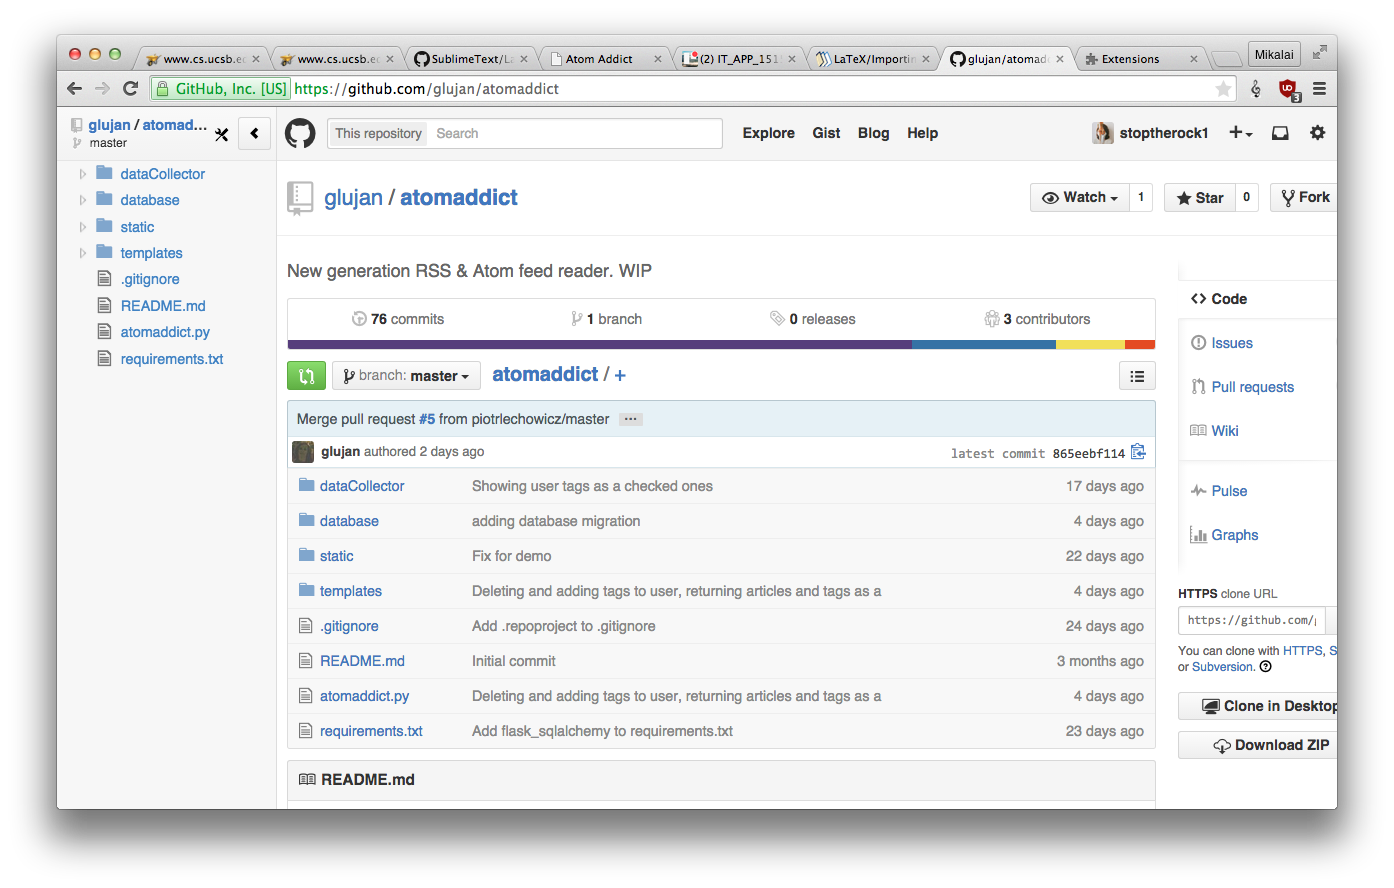
\includegraphics[width=\textwidth]{images/github.png}
    \caption{\textbf{Atomaddict} project repository on \textbf{GitHub}}
    \label{fig:github}
\end{figure}


\subsection{Trello}
Trello is a free web-based project management application originally made by Fog Creek Software in 2011, that spun out to be its own company in 2014.
It operates a freemium business model, as well as being cross-subsidized by other Fog Creek Software products. A basic service is provided free of charge, though a Business Class paid-for service was launched in 2013.

Trello uses the kanban paradigm for managing projects, originally popularized by Toyota in the 1980s for supply chain management. Projects are represented by boards, which contain lists (corresponding to task lists). Lists contain cards (corresponding to tasks). Cards are supposed to progress from one list to the next (via drag-and-drop), for instance mirroring the flow of a feature from idea to implementation. Users can be assigned to cards. Users and boards can be grouped into organizations.

Trello has a variety of work and personal uses including real estate management, software project management, school bulletin boards, lesson planning, and law office case management. A rich API as well as email-in capability enables integration with enterprise systems, or with cloud-based integration services like IFTTT and Zapier.~\cite{wiki:trello}

\begin{figure}[H]
    \centering
    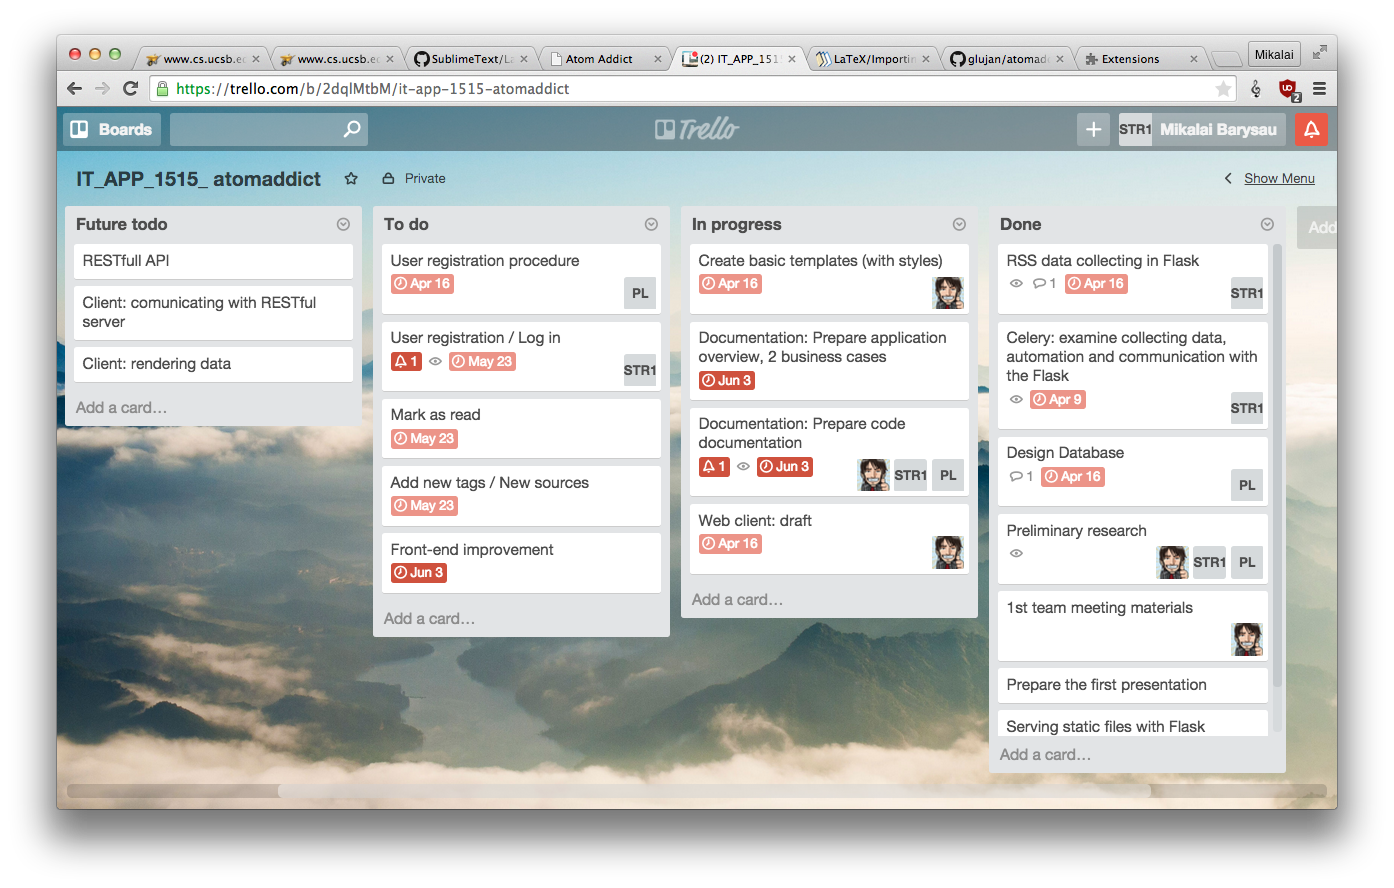
\includegraphics[width=\textwidth]{images/trello.png}
    \caption{\textbf{Atomaddict} project board on \textbf{Trello}}
    \label{fig:trello}
\end{figure}


\subsection{Gantt diagram}

[IMAGE]

\subsection{Work breakdown structure}

[IMAGE]

\section{System diagram}

\begin{figure}[H]
    \centering
    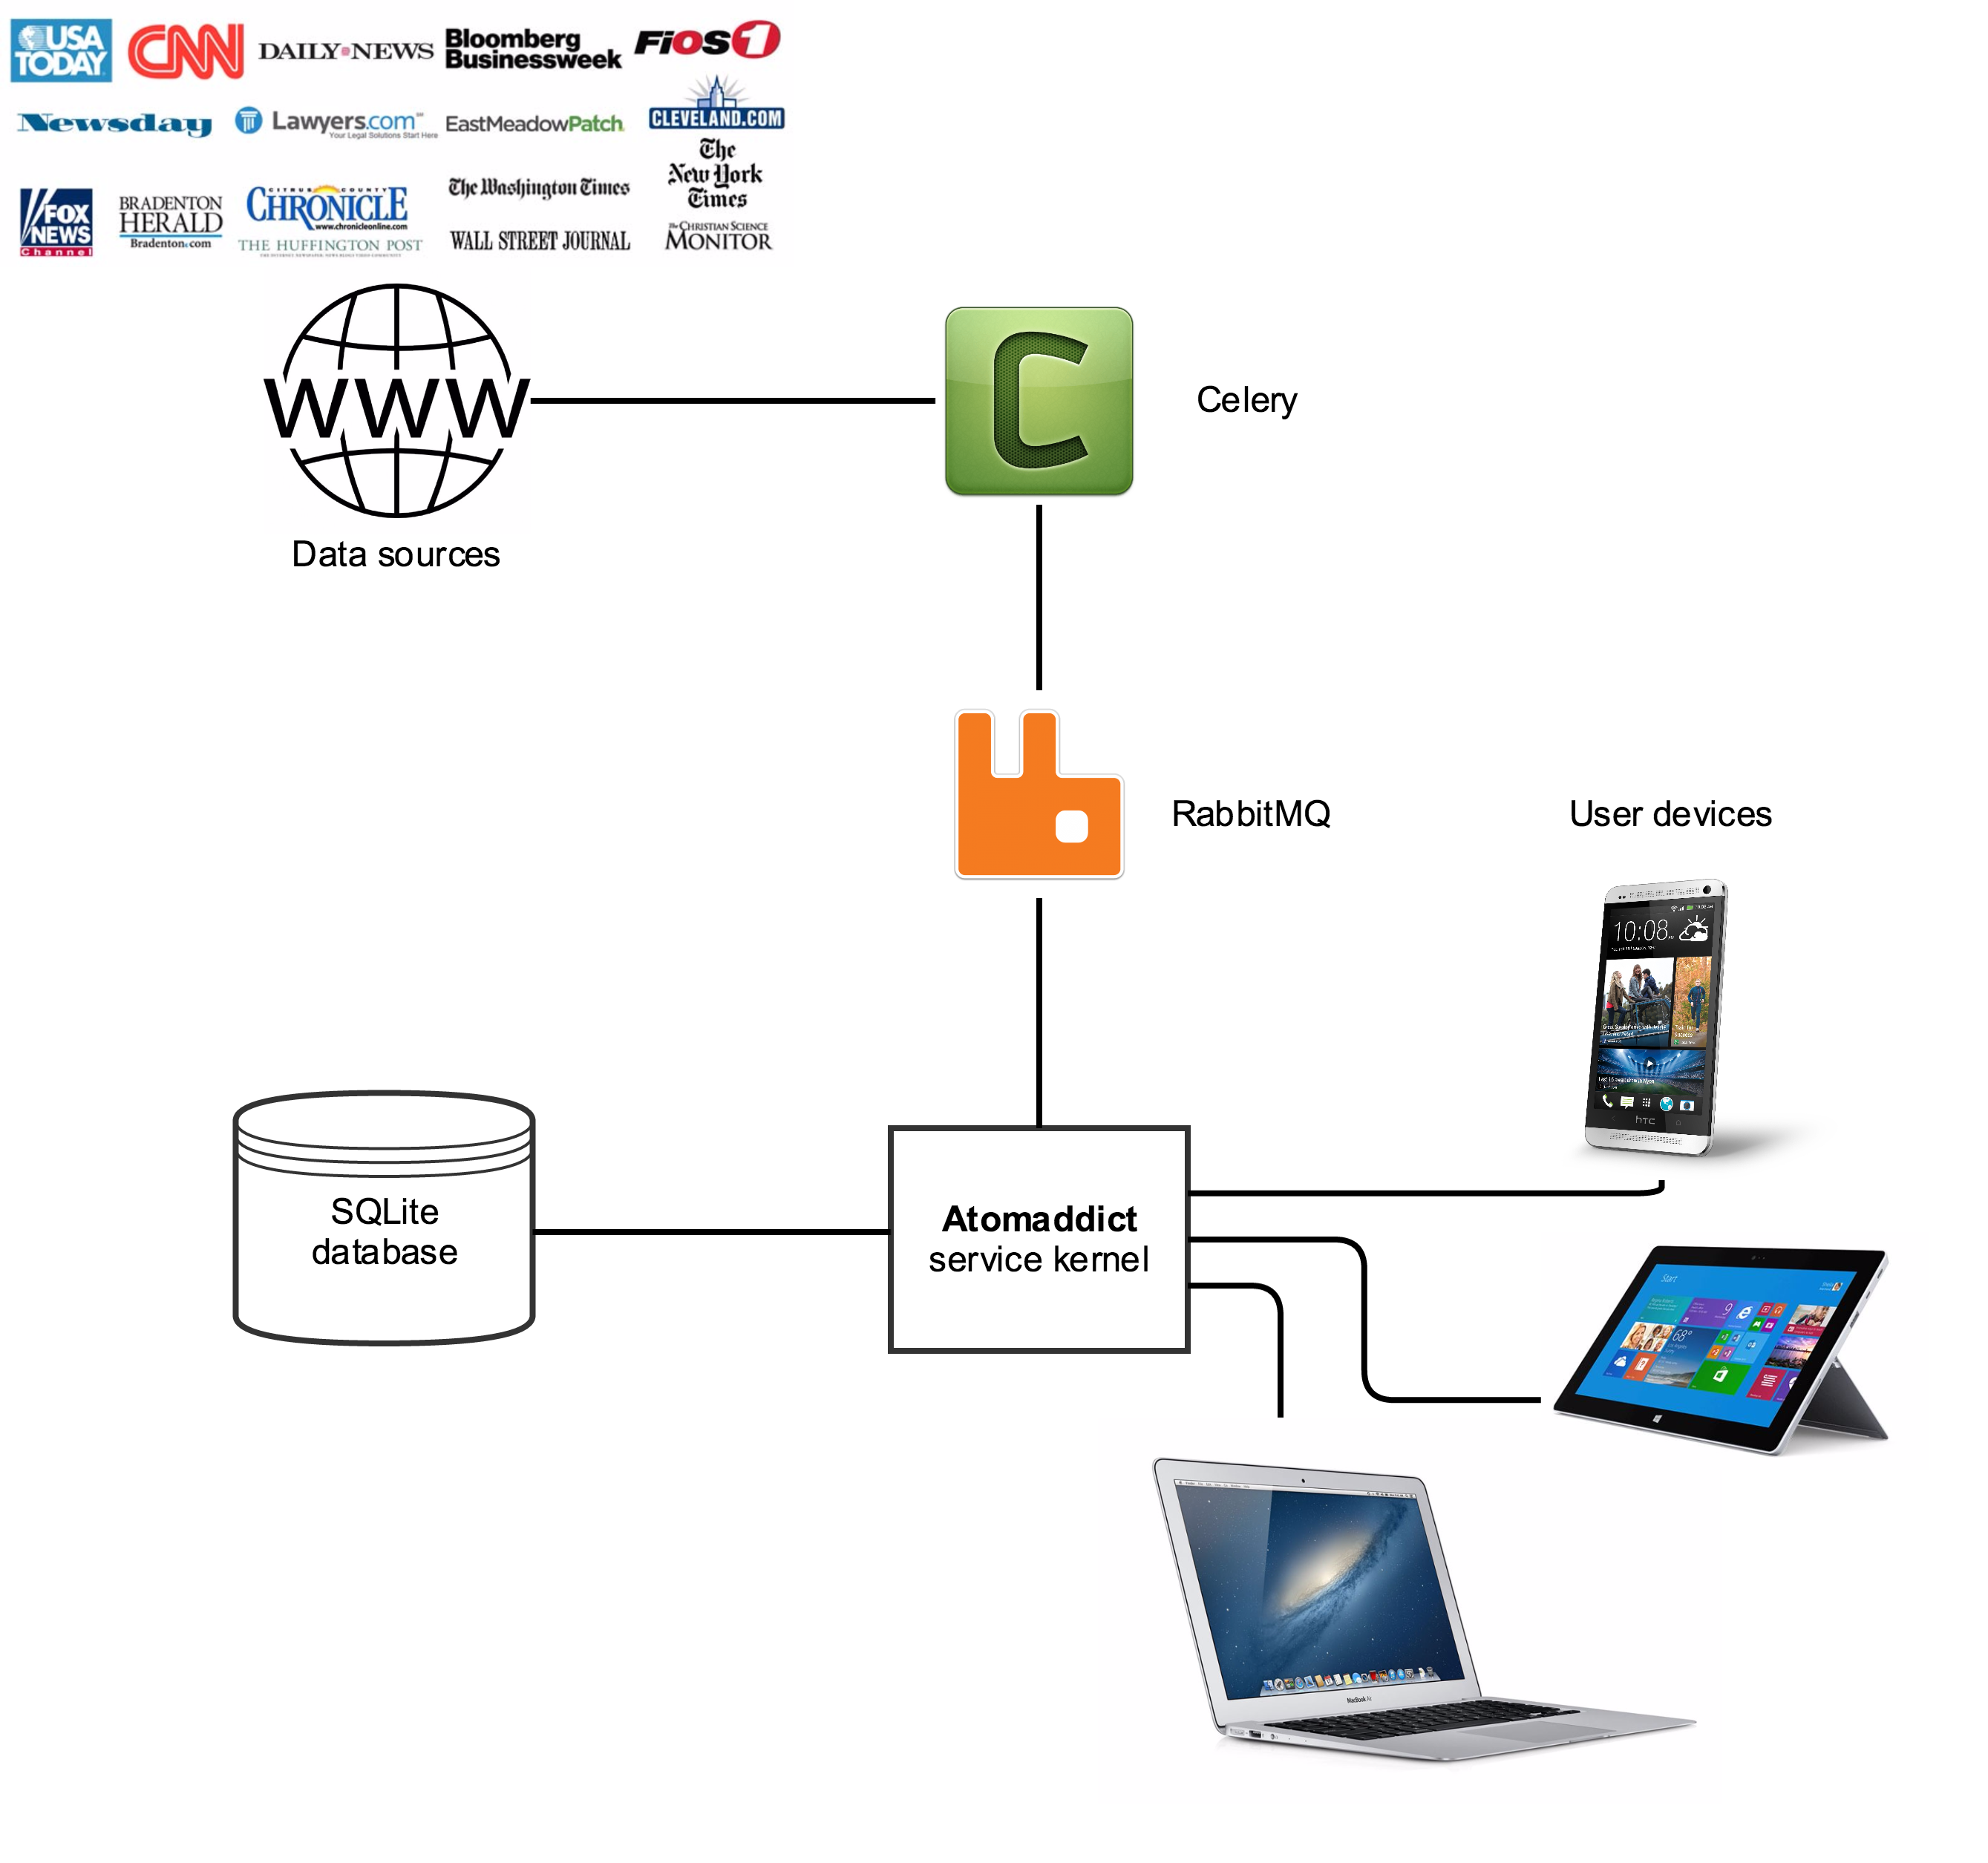
\includegraphics[width=\textwidth]{images/systemDiagram.png}
    \caption{\textbf{Atomaddict} system}
    \label{fig:trello}
\end{figure}

\section{Technologies used in project}
Implementation of \textbf{Atomaddict} project was done in Python, JavaScript, HTML and CSS. Database was created with SQLite engine.

\subsection{Celery}

\subsection{RabbitMQ}

\subsection{Database}

\subsection{Front-end}

\section{Code documentation}

\bibliographystyle{abbrv}
\bibliography{references}

\end{document}
This is never printed
